\documentclass[letterpaper]{article}

\usepackage [english]{babel}
\usepackage [autostyle, english = american]{csquotes}
\MakeOuterQuote{"}
\usepackage{natbib,alifeconf}  %% The order is important
\usepackage{url}
\usepackage{graphicx}
\graphicspath{ {./pictures/} }

\def\imfig#1#2{\begin{figure}[h] \centering \includegraphics[width=\columnwidth]{#1} \caption{#2} \end{figure}}
\def\imfigB#1#2{\begin{figure} \centering \includegraphics[width=\columnwidth]{#1} \caption{#2} \end{figure}}
\def\imfigH#1#2{\begin{figure}[H] \centering \includegraphics[width=\columnwidth]{#1} \caption{#2} \end{figure}}


% *****************
%  Requirements:
% *****************
%
% - All pages sized consistently at 8.5 x 11 inches (US letter size).
% - PDF length <= 8 pages for full papers, <=2 pages for extended
%    abstracts.
% - Abstract length <= 250 words.
% - No visible crop marks.
% - Images at no greater than 300 dpi, scaled at 100%.
% - Embedded open type fonts only.
% - All layers flattened.
% - No attachments.
% - All desired links active in the files.

% Note that the PDF file must not exceed 5 MB if it is to be indexed
% by Google Scholar. Additional information about Google Scholar
% can be found here:
% http://www.google.com/intl/en/scholar/inclusion.html.


% If your system does not generate letter format documents by default,
% you can use the following workflow:
% latex example
% bibtex example
% latex example ; latex example
% dvips -o example.ps -t letterSize example.dvi
% ps2pdf example.ps example.pdf


% For pdflatex users:
% The alifeconf style file loads the "graphicx" package, and
% this may lead some users of pdflatex to experience problems.
% These can be fixed by editing the alifeconf.sty file to specify:
% \usepackage[pdftex]{graphicx}
%   instead of
% \usepackage{graphicx}.
% The PDF output generated by pdflatex should match the required
% specifications and obviously the dvips and ps2pdf steps become
% unnecessary.


% Note:  Some laser printers have a serious problem printing TeX
% output. The use of ps type I fonts should avoid this problem.


\title{They are Very Smart: Genetic-Algorithm-Based Pathfinding in Games}
\author{Joel Tibbetts and Patrick Nuckolls\\
\mbox{}\\
Grinnell College, Grinnell, IA 50112 \\
} % email of corresponding author

% For several authors from the same institution use the same number to
% refer to one address.
%
% If the names do not fit well on one line use
%         Author 1, Author 2 ... \\ {\Large\bf Author n} ...\\ ...
%
% If the title and author information do not fit in the area
% allocated, place \setlength\titlebox{<new height>} after the
% \documentclass line where <new height> is 2.25in


\def\tavs{\textit{They are Very Smart}}
\begin{document}
\maketitle

\begin{abstract}
\tavs~is a destructible tower defense game that explores the viability of short term evolution of neural nets for pathfinding in an adapting adversarial environment.
\end{abstract}

\section{Introduction}
\tavs~is a real-time tower defense game with evolving enemies; which is to say that the player places down towers and other defenses in real time to fend off waves of enemies attempting to destroy the player's "home base." In typical tower defense games, after killing one group of enemies, another comes which is usually stronger than the previous, due to a pre-ordained set of constraints. \tavs~differs from typical tower defense games in that enemy progression is not determined by the game developer, but rather evolves as a result of a genetic algorithm which controls the enemies' damage, movement speed, health, and navigation.

\begin{figure}[h]
	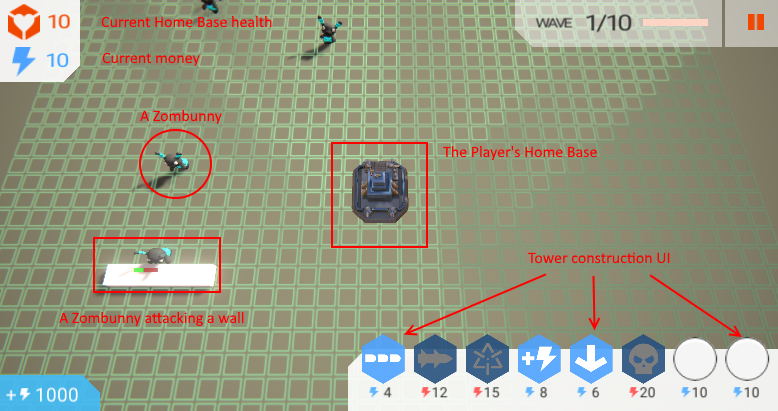
\includegraphics[width=\columnwidth]{InGameLabeled}
	\caption{A screenshot from the game, with various elements labeled}
\end{figure}

In \tavs, player interaction consists of constructing defenses around a central home base. The home base exists in a fixed location in the center of the map, has a set maximum health, and can be damaged by attacks from enemies. Waves of enemies will spawn indefinitely and attempt to destroy the home base. When the health of the home base reaches zero, the game ends.

Players begin the game with an initial sum of money, which can be used to purchase defenses from the tower construction UI (see Figure 1). Defenses are damageable structures which the player may place on any unoccupied square within the defense placement grid.
\imfig{ZoomedOut}{The initial state of the game, showing the home base in the middle of the defense placement grid}

Defenses provide various benefits to the player, such as physically blocking the path of enemies or actively damaging enemies with projectile-based attacks. Some examples of defenses include:
\begin{itemize}
	\item Walls (vertical/horizontal) - inexpensive defenses which block the path of enemies
	\item Machine gun turrets - towers which fire damaging projectiles at nearby enemies
	\item Energy pylons - fragile towers which deal no damage, but instead passively generate income for the player
\end{itemize}

Defenses cost money, which may be gained by killing attacking enemies. As the game progresses, the player may fortify their base by purchasing more expensive defenses and designing complex arrangements of walls and towers in order to thwart enemies.

\pagebreak

\imfig{BaseExample}{An example set of player defenses around the home base}
In \tavs, the player must defend their home base against the aforementioned
onslaught of enemies such as the fearsome Zombunny (see Figure 4). Zombunnies
are driven by a single goal: destruction of the player's home base. Zombunnies
spawn in groups of ten (separated by a slight delay) at the beginning of the
game. Subsequent waves spawn after all members from the previous wave have died.
Zombunnies use a genetic algorithm in conjunction with a recurrent neural
network to evolve a pathfinding algorithm between generations (waves), with the
ultimate goal of dealing damage to (and therefore destroying) the player's base
. Zombunnies can be killed by either taking damage from a player's defenses or
through "starvation." A Zombunny will starve to death if it does not take or
deal damage for a set moved distance. Through this starvation mechanism, the
Zombunnies which survive the longest are ultimately those which interact the
most with the player's defenses. Zombunnies have three
characteristic attributes: health, damage, and movement speed. All three of
these stats are assigned upon spawning as dictated by their genome. Pathfinding
is controlled by a recurrent neural net, whose topology and weight is encoded in
the genome alongside of the characteristic attributes. The neural net evolves on
a wave by wave basis, with those genomes that preform better being more likely
to survive and reproduce than their peers, optimizing for Zombunnies' ability to
achieve their overarching goal of player base destruction. Zombunnies can "see"
nearby entities within a certain radius, including other Zombunnies, player
defenses, and the player's home base (when in range). Based on the combination
of visible inputs, Zombunnies will output a chosen direction which they will
then walk in. This algorithm updates on a tick-by-tick basis. Zombunnies will
damage structures they collide with. Because evolution of the pathfinding neural
net only happens between generations, near the beginning of the game, Zombunnies
will start off with relatively stupid pathfinding which will typically cause the
first few populations to starve to death without dealing any significant damage.
This provides the player with an initial grace period during which they may
build their initial defenses. As time goes on, Zombunnies will evolve towards an
optimal stat distributions of health, damage, and speed, as well as in their
ability to pathfind in such a way as to thwart the player's defenses and end the
game.

\imfig{ZombunnyColliders}{A Zombunny, with attacker and damage colliders highlighted}

%overview
%\begin{itemize}
%    \item Description of tower-defense UI
%    \item Placement of walls vs. towers
%    \item "Spawn points" for zombies
%    \item Central defensible location
%    \item Economy
%    \item Game end/lack thereof
%\end{itemize}

\tavs~was initially inspired by Numantian Games' \textit{They Are Billions}, a
game in which a player must build defenses in order to fend off a zombie
apocalypse. The game features massive numbers of zombies. This project emerged
from an interest in what \textit{They Are Billions} would be like if the zombies
could learn and evolve similarly to a real virus. The result is significantly pared down in
comparison, as the focus has been on zombie evolution as opposed to player
interactivity and enjoyment. However, similarities to \textit{They Are
  Billions} can be seen in the resource management system, the player's defense
of a citadel, and need to fend off the faceless hordes. In contrast,
\textit{They Are Billions} puts additional emphasis on world generation, player
exploration, and narrative elements.

%Insert picture of \textit{They Are Billions} gameplay here.%

\section{Background}
In \tavs, we utilize a basic genetic algorithm to train a recurrent neural
network generated using the Neuroevolution of Augmenting Topologies (NEAT)
method (implemented in the \href{https://www.heatonresearch.com/encog/}{Encog}
framework), which can be found \href{https://sharpneat.sourceforge.net/}{here},
which is a generalized deep-learning library that includes implementations of
a large number of NEAT and HyperNEAT.

NEAT is particularly applicable to our issue because it allows the evolution of different topologies and weights in neural networks at the same time, unlike standard back-propagation learning, and is also well-suited for encoding into a genome for evolution. NEAT works by encoding a function that then generates a neural net, starting out with low complexity of topology, which can then evolve towards more complex topologies.



\section{Tutorial}

\subsection{Running the game}
Our game can be found at
\href{https://github.com/YourFin/They-Are-Very-Smart}{github.com/yourfin/They-Are-Very-Smart},
and downloaded with a standard \texttt{git clone} command. The relevant Unity
scene is then located at
\path{They-Are-Very-Smart/TD/TowerDefence/Assets/Scenes/Levels/Level0/Level0.unity}
Double clicking on this file on any computer with Unity installed will open up
the Unity editor with the context for this paper.

\subsection{Code overview}
\subsubsection{Hyperparameters}
The hyperparameters relevant to playing with how the games are the constants at
the top of \path{Assets/Scripts/Evolution/Genome.cs}, \texttt{HEALTH_SCALE},
\texttt{DAMAGE_SCALE}, and \texttt{MOVEMENT_SCALE}; and at the top of
\path{Assets/Scripts/TowerDefence/Level/GenomeManager.cs}, with
\texttt{POPULATION_SIZE}, \texttt{MUTATION_RATE}, \texttt{GROWTH_RATE},
\texttt{SPAWN_DELAY}, and \texttt{STARTING_TOTAL}. The scale constants in
\path{Genome.cs} change how health, speed, and damage are scaled relative to
each other. \texttt{POPULATION_SIZE} represents the number of genomes (and
therefore zombunnies) in every generation. \texttt{MUTATION_RATE} determines how
much variance there is in everey mutation operation. \texttt{GROWTH_RATE}
Determines how much combined speed, health, and damage is available to be
distributed. \texttt{SPAWN_DELAY} determines how much time passes between spawns
in waves. \texttt{STARTING_TOTAL} determines the total number of stats available
to the zombunnies at the start of the game.

\subsubsection{PolarVector}
The PolarVector class encapsulates the internal representation that we use for storing and passing vectors to the neural net, as well as keeping track of the previous direction a Zombunny was headed during the previous tick. The PolarVector class essentially wraps a float, direction (in degrees) and a float, magnitude, which provides sufficient information to create a new vector in two-dimensional space. The PolarVector class provides some convenient helper methods for converting between Cartesian and Polar coordinate systems, as the Unity engine primarily uses Cartesian coordinates.

%figure 5%
\imfigB{PolarVector1}{The basics of PolarVector}

The implementation details of PolarVector's conversion functions are fairly
trivially derived from math, but it should be noted that all Cartesian
components are encoded as two dimensions of a \texttt{Vector3} as the game takes
place on the X-Z plane (see Figure 6).

\imfigB{PolarVector2}{Conversion functions for PolarVector}

\subsubsection{Genome}
The Genome class encapsulates the data that is stored on a genome-by-genome
basis, provides most of the procedures that deal with their mutation, provides
conversions from their internal state to the game-useful health, speed, and
damage values, and provides an interface to conveniently call the resulting
pathfinding neural net.

\imfigB{Genome1}{Constants and Id for the Genome class}

In Figure 7, we can see the constants that are used to scale a Zombunny's
health, movement speed, and damage, which need to be set manually as discussed
in the hyperparameters sections. The Id field is used as a unique identifier if
genomes need to be looked up, and also ensures that every genome will hash differently.

\imfig{Mutation}{Mutation procedure of the Genome class}

The mutation function in Figure 8 essentially creates a new copy of the current genome, which is then nudged by normally distributed random numbers.

\subsubsection{GenomeManager}

The GenomeManager class keeps track of game-wide genome management, i.e. selection and reproduction, as well as spawning Zombunnies and initiating new waves. The GenomeManager holds onto a collection of all genomes in a wave-by-wave list of hashmaps that map genomes to their fitness. The primary properties of the GenomeManager class can be seen in Figure 9, with various hardcoded constants that can be adjusted to influence general properties of the evolution, as well as the genomeMaps object, which contains the aforementioned collection of all genomes used in the course of evolution thus far.

\imfig{GenomeManagerProperties}{Properties of the GenomeManager class}

The initialization process of GenomeManager (see Figure 10) consists primarily of allocating the containing data structures for the various stages of the genome life cycle, followed by creating a first wave with randomized genomes and zero fitness. It should also be noted that we initialize our ZigguratGaussianSampler here from the Redzen library, which provides a fast way of generating normally-distributed floating-point numbers.

\imfig{GenomeManagerInit}{The GenomeManager initialization process}

Figure 11 shows the NextWave function, which handles the wave-to-wave portions of evolution, i.e. culling and reproduction. It should also be noted that we scramble the Zombunnies, as the Zombunnies get spawned in the order in which they are placed onto the nextWave stack. We scramble the order of the genomes between waves to make sure that evolution doesn't get held up by some side effect of consistent ordering.

\imfig{GenomeManagerNextWave}{The NextWave method of GenomeManager}

The Spawn method, as seen in Figure 12, is called at every SPAWN\_DELAY interval POPULATION\_COUNT times. The function starts by spawning a Zombunny with no genome due to the inability to provide parameters upon GameObject instantiation. Therefore, we set the genome after the fact, popping it off of the toSpawn stack, also adding the ZombieDied function to the removed event on said Zombunny, which allows us to execute code in the context of the GenomeManager upon Zombunny death; namely, ZombunnyDied. ZombunnyDied handles finding the fitness of Zombunnies and adding them to the list of completed genomes, as well as calling NextWave again when the last Zombunny in the wave dies.

\imfig{GenomeManagerSpawn}{Spawning machinery of the GenomeManager class}

\subsubsection{Redzen}

Redzen is a general-purpose utilities library for C\# that contains the fast random function that we use. However, it should be noted that the library as it may be found online at the time of writing does not compile with the older C\# compiler that Unity uses. Thus, we had to manually delete most of the library files and remove underscore digit separators from some numeric constants, as they are a C\# 7 feature. You can find our compatible library at \path{They-Are-Very-Smart/TD/TowerDefense/Assets/Scripts/Util/Redzen}.

\subsubsection{ZombieAgent}

ZombieAgent is a GameObject which determines Zombunny behavior and stats from a genome and keeps track of fitness for each individual Zombunny. To do so, ZombieAgent pulls all the stat-determining values from the genome and applies them upon instantiation, i.e. setting health, damage, and speed as determined by the genome, as well as handling tick-to-tick operations during a Zombunny's lifetime. These tick-to-tick operations include choosing the next movement vector based on the location of nearby GameObjects and agents' current status.

\imfigH{ZombieAgent1}{ZombieAgent class parameters}

In Figure 13, observe that the ZombieAgent class inherits from the Targetable class. Targetable is the parent class for every GameObject in the Action Game Framework, which can be automatically fired upon by ranged weapons, i.e. targeted. This also allows any existing defenses from the default game or any other targeting GameObject from the Action Game Framework to work without extra compatibility code. SINK\_SPEED and SINK\_TIME are constants used for death animation. velocity provides the Zombunny's current velocity for any consumers of the Targetable parent class. LastVelocity stores the previous movement vector as a PolarVector, in a format more congenial to the pathfinding algorithm. Fitness is an interface used to grab the effectiveness of this ZombieAgent at the end of its lifespan by the GenomeManager class. inVision keeps track of all nearby objects that the Zombunny can see for use in its pathfinding algorithm. the alignment is used for purposes of checking whether a Zombunny can damage other GameObjects, while visionCollider and damageCollider are the areas within which a Zombunny can see and deal damage from, respectively. The Rigidbody rigidBody handles physical collisions for movement purposes, while anim keeps track of the Zombunny's animation state, namely walking, idling, or death.

\imfig{ZombieAgentInit}{The Genome, Awake, and Start methods of the ZombieAgent class}

In Figure 14, one can see the Genome, Awake, and Start methods of the
ZombieAgent class. Genome instantiates a Zombunny's Genome object by pulling the
var health from the given Genome, calling the SetMaxHealth and SetHealth
methods, and setting the initial velocity vector to have an initial direction of
$270^\circ$\----that is, in the general direction of the player's base relative
to the spawn location, and magnitude determined by the MovementSpeed variable
from the given Genome. Awake calls the underlying (base) Awake function and adds
custom OnDeath behavior to a Zombunny. Start initializes the inVision HashSet of
Targetable objects, which keeps track of nearby visible GameObjects. In the
unexpected case that genome or lastVelocity are null, Start initializes these to
default values (the "Zero" genome and a default velocity vector).

\imfigH{ZombieAgentVision}{Methods for keeping track of GameObjects entering
  and exiting a Zombunny's visionCollider}

Figure 15 shows the OnTriggerEnter and OnTriggerExit methods of the ZombieAgent
class, which are used in conjunction with a Zombunny's visionCollider to update
the inVision HashSet whenever a GameObject enters or exits the Zombunny's
visionCollider radius.

\imfigH{ZombieAgentUpdateNearby}{The portion of the FixedUpdate method for
determining the position of nearby objects relative to a Zombunny}

Figure 16 shows the functions used to determine the position of GameObjects in
inVision relative to a Zombunny's previous direction vector, stored as a
dictionary of Targetables to PolarVectors. This allows a Zombunny to keep track
of visible GameObjects relative to where it is currently facing.

\imfig{ZombieAgentUpdateMovement}{The function of FixedUpdate that handles
  movement between ticks}

Figure 17 shows the portion of FixedUpdate dedicated to altering a Zombunny's
trajectory from tick to tick, calling the Rotate method of the lastVelocity
PolarVector using the CalculateDirection method of the genome class, taking into
account the Zombunny's previous velocity vector, time alive, current health, and
the aforementioned dictionary of nearby GameObjects.

\imfig{ZombieAgentUpdateDeath}{The portion of FixedUpdate that handles
  death/deletion}

Figure 18 shows the part of the FixedUpdate method which keeps track of Zombunny
death, destroying the Zombunny GameObject at the appropriate time and calling
the relevant death animations. For every tick that a Zombunny is not dead,
FixedUpdate increments timeAlive, which is later used as a factor in
calculating fitness.

\subsubsection{ZombieAttacker}

The ZombieAttacker class (see Figure 19) calls Update on each tick, dealing damage to any item
in toAttack, which is a HashSet of Targetable GameObjects that intersect with
a Zombunny's attack collider (see Figure 4). This way, a Zombunny can attack
multiple GameObjects so long as they intersect with its attack collider. Damage
is applied to items in toAttack by calling their individual takeDamage methods.
Damage dealt is determined by the Zombunny's genome, and is passed as a parameter
to takeDamage.

\imfig{ZombieAttacker}{The Update method of the ZombieAttacker class}



\subsection{Genetic Algorithm}

In \tavs,


%Overview
%\begin{itemize}
%    \item Unity
%    \item Tower Defense tutorial
%    \item Action Game Framework
%    \item Creating custom towers
%    \item Custom scripts
%        \begin{itemize}
%            \item Genome
%            \item ZombieAgent
%            \item GenomeManager
%            \item ZombieAttacker
%        \end{itemize}
%    \item Problems importing packages
%    \item Relevant parts of Encog framework
%        \begin{itemize}
%            \item Manually pulling out Encog training methods for neural nets
%            \item Stealing Softmax function
%        \end{itemize}
%    \item Point array stats system
%    \item Details of genetic algorithm
%        \begin{itemize}
%            \item Mutation
%            \item Keeping track of fitness
%            \item Population management
%            \item Starvation function
%        \end{itemize}
%\end{itemize}


\section{Preliminary Results and Discussion}
Over the course of this project, we learned more about game design than we did
evolutionary algorithms and artificial life. The majority of our time working on
this project was spent dealing with learning the basics of Unity and C\#, which
presented a very significant challenge that we vastly underestimated.

At this time, we are waiting on actual results from our project.
We hope that given a large enough population of Zombunnies, we might see
populations of Zombunnies evolving to counteract players' strategies. Evolution
will likely have little trouble tackling a trivial or consistent player
strategy, like rebuilding the same towers in the same place and
relying heavily on a single tower type, but may have trouble keeping
up with a player that constantly changes strategy over the course of the game.
Our system of softmaxing the genome speed, health, and damage could also
result in progressively larger values relative to the mutation rate, making it
hard for long-evolved high speed value to be traded for damage in the face of
changing player strategies.

Zombunnies will likely evolve around quirks in the way the
game is organized. The primary example would be having health that is just above
multiples of tower damage, allowing it to sustain an additional hit with
insignificant investment in the health stat. This particular problem could be
solved by having towers deal damage with slight randomness, but there likely
exist similar problems that have not been considered.

Players, on the other hand, may also learn to optimize around our implementation
of evolution. Conceivably clever players could develop two very different
strategies ahead of time. The player would first implement the weaker strategy,
and as soon as the Zombunnies have deeply rooted themselves in the local maximum
versus that strategy, the strategy could be changed to the second strategy,
leaving the Zombunnies unable to easily adapt to the new strategy.

Solving these problems would probably involve moving towards more complicated
models of selection and reproduction than our current keep \(n\) percent,
asexually reproduce the best genomes and then do a straight pass of mutation.
Moving to a system where reproductive resources are distributed according to the
Z-score (standard deviations from the mean) or similar of fitness that give more
reproductive power to individual that more drastically improve on the status quo
could allow for a system that reacts more strongly to change. Another option
could be coding part of the mutation rate in genomes to allow evolution to
determine it's own speed. The two previous approaches could even be combined for
as dynamic an evolution environment as possible.

Sexual (genderless) reproduction could also be introduced as a way of trying to
incentivize diversity. Plain sexual reproduction without any further restrictions
could allow good traits that evolve in parallel to be combined into a single
individual with the benefits of both, which has fairly obvious advantages.
This simple approach to sexual reproduction could, however, force a single
species to dominate quickly depending on how well neural net parameters combine,
as it could easily be the case that two disparately evolving neural nets combine
into a total dud, despite having fit parents. One way around that would be to
condition reproduction on similarity, such genomes are more likely to reproduce
with those that are structurally similar. Another approach would be to allow
genomes to determine mating preference based on other genomes' content and
fitness, and then run them through a tournament to determine mates. This would
have the additional benefit of allowing emergent behavior that has not been
conceived of in this speculation.

Conceptually, evolving neural nets instead of using backpropagation
has the massive benefit of not worrying about how to differentiate and nicely
back-propagate the reward/fitness function to learn, which opens up the
possibility to drop in a neural net to replace any function in a learning
environment; on a larger timescale, the selection tournament process itself
could modeled with a recurrent neural network, and evolved over multiple plays
of the game.

Allowing the Zombunnies to keep track of what they learn from game to game could
be useful as a ``hard mode'' should the base game be too easy, perhaps with the
additional information passed to the navigation function of the round. In an actual game
using this technology to evolve AI, this could be expanded to the entire
playerbase training a single pathfinding algorithm that is then redistributed to
each client, and perhaps even takes in all previous player game history as
additional input. The missing backpropagation requirement opens up
any function to becoming an neural net, and with any input.

\section{Conclusion}
\begin{itemize}
    \item Synopsis of project
    \item Future work and next steps
\end{itemize}

\section{Acknowledgments}
\begin{itemize}
    \item Use of multiple tutorials/repositories
    \begin{itemize}
        \item Encog Machine Learning Framework
        \item Unity Tower Defense Tutorial
        \item Unity Action Game Shooter Tutorial
        \item Redzen repository for normal random numbers
    \end{itemize}
\end{itemize}

\footnotesize
\bibliographystyle{apalike}
\bibliography{bibliography} % replace by the name of your .bib file

\end{document}
